\documentclass[11pt]{amsart}
\usepackage[a4paper,margin=1in]{geometry}
\usepackage{amssymb}
\usepackage{booktabs}
\usepackage{tikz}
\usetikzlibrary{patterns}
\usepackage[font=small,labelfont=bf]{caption}
\usepackage[hidelinks]{hyperref}

\colorlet{copper}{orange!75!black}
\colorlet{inkmuted}{black!60}
\tikzset{book/thin/.style={black!55, line width=0.4pt}}

\newtheorem{theorem}{Theorem}
\newtheorem{lemma}[theorem]{Lemma}
\theoremstyle{remark}
\newtheorem{remark}[theorem]{Remark}

\title{A Sequence That Looks Back Half Way}
\author{Vamshi Jandhyala}
\address{London, United Kingdom}
\email{vamshi.jandhyala@gmail.com}

\begin{document}

\begin{abstract}
Let $a_1=1$, $a_n=a_{n-1}$ for even $n$ and $a_n=a_{n-1}-a_{(n-1)/2}/n$ for odd $n$. A question on Mathematics Stack Exchange asked for the constant $A$ with $na_n\to A$, and a commenter conjectured $A=1/(1-\ln2)$ from its digits. We prove this. The proof rests on an exact identity, $na_n=1+\sum_{n/2\le k<n}a_k$, which turns the recurrence into an average over a window of total weight tending to $\ln2<1$. Every step is formally verified in Lean~4.
\end{abstract}

\maketitle

\section{The question}

Start with $a_1=1$ and build a sequence of rationals by two rules. At an even step nothing happens; at an odd step the sequence drops by a fraction of an earlier term:
\[
a_n=\begin{cases} a_{n-1}, & n\text{ even},\\[2pt] a_{n-1}-\dfrac1n\,a_{(n-1)/2}, & n\text{ odd}.\end{cases}
\]
The first terms are $1,1,\tfrac23,\tfrac23,\tfrac7{15},\tfrac7{15},\tfrac{13}{35}$, and the sequence falls like $A/n$ with $A\approx3.2588913$. The user AAK asked on Mathematics Stack Exchange in August 2023 (question 4748129) for a way to compute $A$ and an expression for it in known constants; the sequence came from a branching process in a random environment. The same day Tian Vlasic searched the digits and suggested $A=1/(1-\ln2)=3.2588913\ldots$, and Gary derived the equation $[(1-x)F(x)]'=1-F(x^2)$ for the generating function $F$ and observed that $-\log(1-x)/(1-\ln2)$ satisfies it asymptotically as $x\to1^-$.

\begin{theorem}\label{thm:main}
$\displaystyle\lim_{n\to\infty}n\,a_n=\frac1{1-\ln2}$.
\end{theorem}

This is the coefficient version of Gary's remark, reached without a Tauberian argument. The odd-indexed terms have numerators 1, 2, 7, 13, 281, 530, 29599, \dots\ and denominators 1, 3, 15, 35, 945, 2079, 135135, \dots; neither sequence is in the OEIS (searched 10 October 2026).

\section{The window identity}

Let the \emph{window} of $n$ be $W_n=\{k\in\mathbb Z:\ n/2\le k<n\}$, so $W_7=\{4,5,6\}$, $W_8=\{4,5,6,7\}$ and $W_1=\emptyset$.

\begin{lemma}\label{lem:window}
For every $n\ge1$, $\displaystyle n\,a_n=1+\sum_{k\in W_n}a_k$.
\end{lemma}

\begin{proof}
Let $Q_n=na_n-\sum_{k\in W_n}a_k$, so $Q_1=1$. Passing from $W_{n-1}$ to $W_n$ adds the index $n-1$, and removes the bottom index $(n-1)/2$ exactly when $n$ is odd. Hence $Q_n-Q_{n-1}=n(a_n-a_{n-1})+[n\text{ odd}]\,a_{(n-1)/2}$, which is $0$ by the recurrence in both cases.
\end{proof}

For $n=7$ the lemma reads $7\cdot\tfrac{13}{35}=1+\tfrac23+\tfrac7{15}+\tfrac7{15}$. By induction it also shows $a_n>0$: the right-hand side is at least $1$ when the earlier terms are positive. Figure~\ref{fig:window24} shows the identity for $n=24$.

\begin{figure}[ht]
\centering
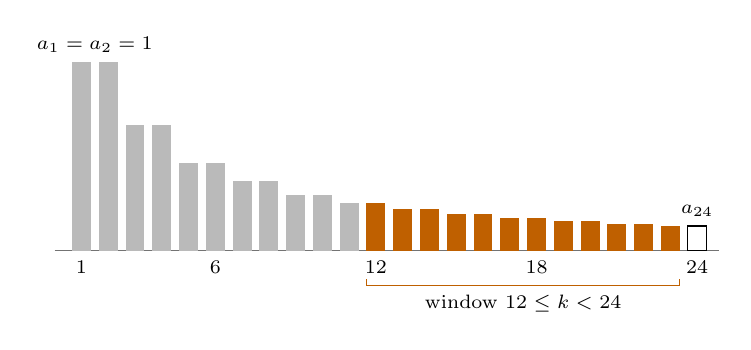
\begin{tikzpicture}
  \draw[book/thin] (0,0) -- (8.432,0);
\fill[inkmuted!45] (0.220,0) rectangle (0.460,2.400);
\fill[inkmuted!45] (0.560,0) rectangle (0.800,2.400);
\fill[inkmuted!45] (0.900,0) rectangle (1.140,1.600);
\fill[inkmuted!45] (1.240,0) rectangle (1.480,1.600);
\fill[inkmuted!45] (1.580,0) rectangle (1.820,1.120);
\fill[inkmuted!45] (1.920,0) rectangle (2.160,1.120);
\fill[inkmuted!45] (2.260,0) rectangle (2.500,0.891);
\fill[inkmuted!45] (2.600,0) rectangle (2.840,0.891);
\fill[inkmuted!45] (2.940,0) rectangle (3.180,0.714);
\fill[inkmuted!45] (3.280,0) rectangle (3.520,0.714);
\fill[inkmuted!45] (3.620,0) rectangle (3.860,0.612);
\fill[copper] (3.960,0) rectangle (4.200,0.612);
\fill[copper] (4.300,0) rectangle (4.540,0.526);
\fill[copper] (4.640,0) rectangle (4.880,0.526);
\fill[copper] (4.980,0) rectangle (5.220,0.466);
\fill[copper] (5.320,0) rectangle (5.560,0.466);
\fill[copper] (5.660,0) rectangle (5.900,0.414);
\fill[copper] (6.000,0) rectangle (6.240,0.414);
\fill[copper] (6.340,0) rectangle (6.580,0.376);
\fill[copper] (6.680,0) rectangle (6.920,0.376);
\fill[copper] (7.020,0) rectangle (7.260,0.342);
\fill[copper] (7.360,0) rectangle (7.600,0.342);
\fill[copper] (7.700,0) rectangle (7.940,0.316);
\draw (8.040,0) rectangle (8.280,0.316);
\node[below, font=\scriptsize] at (0.340,0) {1};
\node[below, font=\scriptsize] at (2.040,0) {6};
\node[below, font=\scriptsize] at (4.080,0) {12};
\node[below, font=\scriptsize] at (6.120,0) {18};
\node[below, font=\scriptsize] at (8.160,0) {24};
\draw[copper] (3.960,-0.36) -- (3.960,-0.44) -- (7.940,-0.44) -- (7.940,-0.36);
\node[below, font=\scriptsize] at (5.950,-0.44) {window $12\le k<24$};
\node[above, font=\scriptsize] at (8.160,0.316) {$a_{24}$};
\node[above, font=\scriptsize] at (0.510,2.400) {$a_1=a_2=1$};

\end{tikzpicture}
\caption{The terms $a_k$ for $k\le24$. The copper bars are the window $W_{24}=\{12,\dots,23\}$. Lemma~\ref{lem:window} says that twenty-four copies of the last bar (hatched) exceed the copper bars by exactly $1$.}
\label{fig:window24}
\end{figure}

Write $c_n=na_n$. Since $a_k=c_k/k$, the identity becomes
\begin{equation}\label{eq:c}
c_n=1+\sum_{k\in W_n}\frac{c_k}{k}.
\end{equation}
So $c_n$ is $1$ plus a weighted sum of earlier values of $c$, with total weight
\[
s_n=\sum_{k\in W_n}\frac1k\ \approx\ \int_{n/2}^{n}\frac{dx}{x}=\ln 2 .
\]
If $c_n$ has a limit $A$, then $A=1+A\ln2$, which is the conjectured constant. The proof makes this honest, and the only thing it needs about the weights is their limit.

\begin{lemma}\label{lem:weights}
$s_n\to\ln2$.
\end{lemma}

\begin{proof}
With $N=n-1$ and $t=\lceil n/2\rceil-1$ the window is $\{t+1,\dots,N\}$, so $s_n=H_N-H_t$, a difference of harmonic numbers. Since $H_m-\ln m$ tends to Euler's constant,
\[
s_n=(H_N-\ln N)-(H_t-\ln t)+\ln\frac{N}{t}\ \longrightarrow\ \ln 2,
\]
because $2t\le N\le2t+1$.
\end{proof}

\section{Proof of the theorem}

\emph{Boundedness.} By Lemma~\ref{lem:weights}, $s_n\le\tfrac34$ for all $n\ge N_0$. Let $B$ be the larger of $4$ and $c_1+\dots+c_{N_0}$. Then $c_n\le B$ for $n\le N_0$, and if $c_k\le B$ for all $k<n$ with $n>N_0$, then \eqref{eq:c} gives $c_n\le1+s_nB\le1+\tfrac34B\le B$. So $0<c_n\le B$ for all $n$.

\emph{The error.} Let $A=1/(1-\ln2)$, so that $A=1+A\ln2$, and put $e_n=c_n-A$. Substituting $c_k=A+e_k$ into \eqref{eq:c},
\begin{equation}\label{eq:e}
e_n=\sum_{k\in W_n}\frac{e_k}{k}+A\,(s_n-\ln2),
\end{equation}
so if $|e_k|\le R$ throughout the window, then
\[
|e_n|\le s_n R+\delta_n,\qquad \delta_n=A\,|s_n-\ln2|.
\]
For $n\ge N_0$ this is at most $\tfrac34R+\delta_n$, and $\delta_n\to0$. The error in the window shrinks by a factor $\tfrac34$, up to a vanishing term, each time we pass to indices twice as large.

\begin{proof}[Proof of Theorem~\ref{thm:main}]
The errors are bounded, say $|e_n|\le M$. Given $\eta>0$, choose $N_1$ with $\delta_n\le\eta$ for $n\ge N_1$. We claim that for each $j\ge0$ there is an $N$ with
\[
|e_n|\le(\tfrac34)^jM+4\eta\qquad(n\ge N).
\]
For $j=0$ this holds with $N=0$. If it holds for $j$ with threshold $N$, take $n\ge\max(2N+1,N_0,N_1)$. Every index in $W_n$ is at least $N$, so the window bound applies with $R=(\tfrac34)^jM+4\eta$, and
\[
|e_n|\le\tfrac34\bigl((\tfrac34)^jM+4\eta\bigr)+\eta=(\tfrac34)^{j+1}M+4\eta .
\]
Choosing $j$ large and $\eta$ small makes the bound as small as we like, so $e_n\to0$ and $c_n\to A$.
\end{proof}

The proof uses $\ln2<1$ twice, in the boundedness step and in the contraction. That is where the window of half the indices matters: a window from $n/3$ to $n$ would carry weight $\ln3>1$, and the argument would prove nothing.

\begin{figure}[ht]
\centering
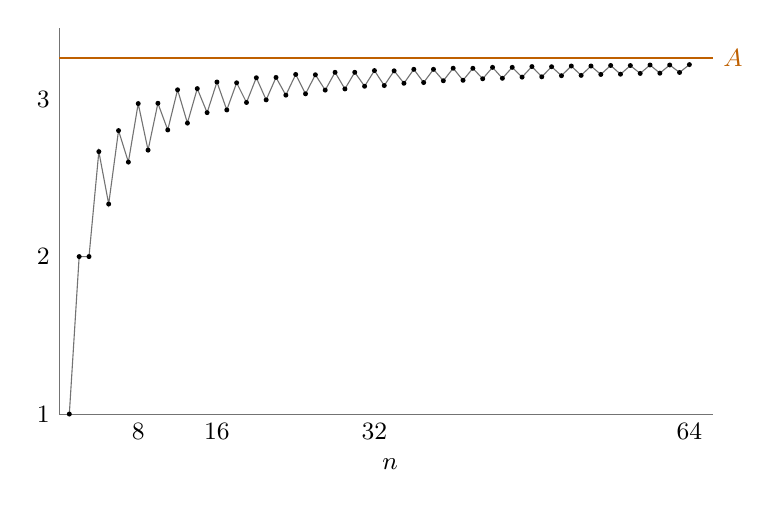
\begin{tikzpicture}
  \draw[book/thin] (0,0) -- (8.3,0);
  \draw[book/thin] (0,0) -- (0,4.9);
  \draw[copper, thick] (0,4.518) -- (8.3,4.518) node[right, font=\small] {$A$};
  \draw[book/thin] (0.125,0.000) -- (0.250,2.000) -- (0.375,2.000) -- (0.500,3.333) -- (0.625,2.667) -- (0.750,3.600) -- (0.875,3.200) -- (1.000,3.943) -- (1.125,3.352) -- (1.250,3.947) -- (1.375,3.608) -- (1.500,4.118) -- (1.625,3.695) -- (1.750,4.133) -- (1.875,3.828) -- (2.000,4.217) -- (2.125,3.862) -- (2.250,4.207) -- (2.375,3.957) -- (2.500,4.271) -- (2.625,3.990) -- (2.750,4.275) -- (2.875,4.050) -- (3.000,4.313) -- (3.125,4.067) -- (3.250,4.309) -- (3.375,4.114) -- (3.500,4.340) -- (3.625,4.129) -- (3.750,4.340) -- (3.875,4.163) -- (4.000,4.362) -- (4.125,4.172) -- (4.250,4.359) -- (4.375,4.201) -- (4.500,4.378) -- (4.625,4.210) -- (4.750,4.378) -- (4.875,4.233) -- (5.000,4.392) -- (5.125,4.239) -- (5.250,4.391) -- (5.375,4.258) -- (5.500,4.403) -- (5.625,4.264) -- (5.750,4.403) -- (5.875,4.279) -- (6.000,4.413) -- (6.125,4.283) -- (6.250,4.411) -- (6.375,4.297) -- (6.500,4.420) -- (6.625,4.301) -- (6.750,4.420) -- (6.875,4.313) -- (7.000,4.427) -- (7.125,4.316) -- (7.250,4.426) -- (7.375,4.326) -- (7.500,4.433) -- (7.625,4.329) -- (7.750,4.433) -- (7.875,4.338) -- (8.000,4.438);
\fill (0.125,0.000) circle (0.9pt);
\fill (0.250,2.000) circle (0.9pt);
\fill (0.375,2.000) circle (0.9pt);
\fill (0.500,3.333) circle (0.9pt);
\fill (0.625,2.667) circle (0.9pt);
\fill (0.750,3.600) circle (0.9pt);
\fill (0.875,3.200) circle (0.9pt);
\fill (1.000,3.943) circle (0.9pt);
\fill (1.125,3.352) circle (0.9pt);
\fill (1.250,3.947) circle (0.9pt);
\fill (1.375,3.608) circle (0.9pt);
\fill (1.500,4.118) circle (0.9pt);
\fill (1.625,3.695) circle (0.9pt);
\fill (1.750,4.133) circle (0.9pt);
\fill (1.875,3.828) circle (0.9pt);
\fill (2.000,4.217) circle (0.9pt);
\fill (2.125,3.862) circle (0.9pt);
\fill (2.250,4.207) circle (0.9pt);
\fill (2.375,3.957) circle (0.9pt);
\fill (2.500,4.271) circle (0.9pt);
\fill (2.625,3.990) circle (0.9pt);
\fill (2.750,4.275) circle (0.9pt);
\fill (2.875,4.050) circle (0.9pt);
\fill (3.000,4.313) circle (0.9pt);
\fill (3.125,4.067) circle (0.9pt);
\fill (3.250,4.309) circle (0.9pt);
\fill (3.375,4.114) circle (0.9pt);
\fill (3.500,4.340) circle (0.9pt);
\fill (3.625,4.129) circle (0.9pt);
\fill (3.750,4.340) circle (0.9pt);
\fill (3.875,4.163) circle (0.9pt);
\fill (4.000,4.362) circle (0.9pt);
\fill (4.125,4.172) circle (0.9pt);
\fill (4.250,4.359) circle (0.9pt);
\fill (4.375,4.201) circle (0.9pt);
\fill (4.500,4.378) circle (0.9pt);
\fill (4.625,4.210) circle (0.9pt);
\fill (4.750,4.378) circle (0.9pt);
\fill (4.875,4.233) circle (0.9pt);
\fill (5.000,4.392) circle (0.9pt);
\fill (5.125,4.239) circle (0.9pt);
\fill (5.250,4.391) circle (0.9pt);
\fill (5.375,4.258) circle (0.9pt);
\fill (5.500,4.403) circle (0.9pt);
\fill (5.625,4.264) circle (0.9pt);
\fill (5.750,4.403) circle (0.9pt);
\fill (5.875,4.279) circle (0.9pt);
\fill (6.000,4.413) circle (0.9pt);
\fill (6.125,4.283) circle (0.9pt);
\fill (6.250,4.411) circle (0.9pt);
\fill (6.375,4.297) circle (0.9pt);
\fill (6.500,4.420) circle (0.9pt);
\fill (6.625,4.301) circle (0.9pt);
\fill (6.750,4.420) circle (0.9pt);
\fill (6.875,4.313) circle (0.9pt);
\fill (7.000,4.427) circle (0.9pt);
\fill (7.125,4.316) circle (0.9pt);
\fill (7.250,4.426) circle (0.9pt);
\fill (7.375,4.326) circle (0.9pt);
\fill (7.500,4.433) circle (0.9pt);
\fill (7.625,4.329) circle (0.9pt);
\fill (7.750,4.433) circle (0.9pt);
\fill (7.875,4.338) circle (0.9pt);
\fill (8.000,4.438) circle (0.9pt);

  \foreach \n in {8,16,32,64} \node[below, font=\small] at (\n/8,0) {$\n$};
  \foreach \c in {1,2,3} \node[left, font=\small] at (0,{2*(\c-1)}) {$\c$};
  \node[below, font=\small] at (4.2,-0.45) {$n$};
\end{tikzpicture}
\caption{$c_n=na_n$ for $n\le64$, climbing towards $A=1/(1-\ln2)$. In this range it rises at every even step, where $c_n=\tfrac{n}{n-1}c_{n-1}$, and falls at every odd step.}
\label{fig:cn}
\end{figure}

\begin{remark}
The rate is not proved here, but the numbers are regular. Iterating to $n=2\times10^6$, $n(c_n-A)$ settles at $-2.58870$ for even $n$ and $-5.84759$ for odd $n$. The two constants differ by $A$ to the digits shown, which the even step explains: $c_{2m}-c_{2m-1}=c_{2m-1}/(2m-1)\approx A/(2m)$. In a continuous model, with $n=e^\tau$, identity~\eqref{eq:c} becomes the delay equation $c(\tau)=1+\int_{\tau-\ln2}^{\tau}c$, whose perturbations $e^{\lambda\tau}$ satisfy $\lambda=1-2^{-\lambda}$. The root $\lambda=-1$ is a perturbation of size $1/n$ that solves the homogeneous equation by itself, which suggests that the coefficient of $1/n$ depends on the whole early history of the sequence and has no closed form.
\end{remark}

\section{Verification}

Lemmas~\ref{lem:window} and~\ref{lem:weights}, the boundedness of $c_n$, identity~\eqref{eq:e}, the contraction argument and Theorem~\ref{thm:main} are proved in Lean~4 with Mathlib~\cite{mathlib}, using only the standard axioms; Lemma~\ref{lem:weights} uses Mathlib's limit of $H_m-\ln m$. A Python program checks the window identity in exact rational arithmetic for $n\le3000$ and iterates to $n=2\,000\,001$ for the remark, and catches three planted errors in the recurrence and the window. Code and Lean files are at~\cite{repo}.

\section*{Acknowledgments}

The question is by the Mathematics Stack Exchange user AAK, the constant was conjectured by Tian Vlasic, and the generating-function remark is Gary's. The proof, the computations and the Lean formalisation were carried out with Claude Opus~5.5 (Anthropic); an answer with this proof was posted to the question (answer 5150836). The author is responsible for the content.

\begin{thebibliography}{9}
\bibitem{MSE} AAK, \emph{Asymptotics of sequence of rational numbers}, Mathematics Stack Exchange question 4748129 (2023), \url{https://math.stackexchange.com/q/4748129}.
\bibitem{mathlib} The mathlib Community, \emph{The Lean mathematical library}, in: Proc. 9th ACM SIGPLAN Int. Conf. on Certified Programs and Proofs (CPP 2020), 367--381.
\bibitem{repo} V.~Jandhyala, code and Lean proofs, \url{https://github.com/jvvk/mathematics/tree/main/half-window-sequence}.
\end{thebibliography}

\end{document}
